\listfiles

\documentclass[11.5pt,a4paper]{article}

\usepackage{amsthm,amssymb,amsmath}
\usepackage{wasysym}
\usepackage{mathtools}

\newcommand\persiangloss[2]{#1\dotfill\lr{#2}\\}

\newcommand{\nocontentsline}[3]{}
\newcommand{\tocless}[2]{\bgroup\let\addcontentsline=\nocontentsline#1{#2}\egroup}
\usepackage[bottom]{footmisc}
\usepackage{indentfirst}

\usepackage{caption}

\usepackage{graphicx}
\usepackage{subcaption}
\usepackage{array}
\usepackage{adjustbox}
\usepackage{tablefootnote}
\usepackage{amsfonts}
\usepackage{amssymb}
\usepackage{yfonts}
\usepackage{subcaption}
\usepackage{relsize}

\usepackage{xcolor,colortbl}
%\definecolor{Gray}{gray}{0.90}
%\definecolor{LGray}{gray}{0.95}
\usepackage{color}

\usepackage{listings}

\usepackage[scr=euler,bb=ams]{mathalfa}


\usepackage[pagebackref=false,colorlinks,linkcolor=blue,citecolor=magenta]{hyperref}

\usepackage[a4paper]{geometry} 
\geometry{a4paper,tmargin=3.5cm, bmargin=2.5cm, lmargin=2cm, rmargin=2.5cm, headheight=3em, headsep=1.5cm, footskip=1cm} 

\usepackage{xepersian}
\settextfont[Scale=1]{B Nazanin}
\setlatintextfont[Scale=1]{Georgia}

%\settextfont[Scale=1.1]{B Zar}

%\DefaultMathsDigits
\setdigitfont{XB Zar}

\defpersianfont\titr[Scale=1]{B Titr}
%\defpersianfont\nastaliq[Scale=1.5]{IranNastaliq}
%\defpersianfont\traffic[Scale=1]{B Traffic}
%\defpersianfont\yekan[Scale=1]{B Yekan}
%\defpersianfont\traffic[Scale=1]{XB Roya}
%\defpersianfont\yekan[Scale=1]{XB Kayhan}
%%%%%%%%%%%%%%%%%%%%%%%%%%%%%%%%%%%%%%%%%%%%%%%%%%%
\usepackage{zref-perpage}
\zmakeperpage{footnote}

%%%%%%%%%%%%%%%%%%%%%%%%%%%%%%%%%%%%%%%%%%%%%%%%%%%
\newcommand{\enfootnote}[1]{\footnote{\lr{#1}}}
\newcommand\numberthis{\addtocounter{equation}{1}\tag{\theequation}}


%%%%%%%%%%%%%%%%%%%%%%%%%%%%%%%%%%%%%%%%%%%%%%%%%%%

\definecolor{customblue}{RGB}{235,241,245}
\definecolor{light-gray}{gray}{0.95}
\lstdefinestyle{C++Style}{%
  backgroundcolor=\color{customblue},
  breaklines=true,
  basicstyle=\footnotesize\ttfamily,
  keywordstyle=\color{blue},
  commentstyle=\color{OliveGreen}\textit,
  stringstyle=\color{red},
  numbers=left,
  numberstyle={\tiny\lr},
  showspaces = false,
  showstringspaces = false,
  tabsize = 2,
  frame=single,
  xleftmargin=5pt,
  xrightmargin=3pt,
  language =  C++,
  aboveskip = 20pt,
  rulecolor=\color{black},
%  captiondirection=RTL,
}

\lstnewenvironment{C++Code}[1][]
{%
  \lstset{style=C++Style, #1}%
}{%
}

\def\lstlistingname{برنامه}

%%%%%%%%%%%%%%%%%%%%%%%%%%%%%%%%%%%%%%%%%%%%%%%%%%%
\begin{document}

\thispagestyle{empty}
\vspace*{-28mm}
\centerline{
\includegraphics[height=5cm]{Imgs/ceit_logo.png}}

\begin{center}
%دستوری برای کم کردن فاصله بین لوگو و خط پایین آن
\vspace{-2mm}
{\LARGE
{
دانشکده مهندسی کامپیوتر و فن‌آوری اطلاعات\\	
دانشگاه صنعتی امیرکبیر	
}
%دستوری برای تعیین فاصله بین دو خط
\\[2.1cm]
}

{\large
\textbf{گزارش پروژه دسته‌بندی تصاویر ایستای حالات دست}
\\[2cm]

استاد درس:
\\[.5cm]
{\Large
دکتر صفابخش}
\\[1.5cm]
\large 
نام دانشجو:
\\[.5cm]
{\Large
احمد اسدی}
\\[.5cm]
۹۴۱۳۱۰۹۱
\\[1.5cm]
}
%دستوری برای تعیین فاصله بین خطوط (نه دو خط) و تا وقتی که مقدار آن تغییر نکند، فاصله بین خطوط، همین مقدار است.

{\large
تیرماه 1395
}
\end{center}

\newpage
\baselineskip=1cm
\tocless\tableofcontents

\newpage
\baselineskip=0.75cm
\pagenumbering{arabic}

%%%%%%%%%%%%%%%%%%%%%%%%%%%%%%%%%%%%%%%%%%%%%%%%%%%%%%%%%%%%%%%%%%%%%%%%%%%%%%%%%%%
\section{ مقدمه}
تشخیص حالت دست از روی تصاویر، یکی از پرکارترین و فعال‌ترین حوزه‌های پژوهشی در زمینه ارتباط انسان و رایانه\enfootnote{Human Computer Interaction (HCI)} است. تعامل انسان و رایانه با استفاده از حرکات و حالات دست، علاوه بر این‌که حس بهتری به کاربر در هنگام کار با سیستم‌های رایانه‌ای می‌بخشد، راه‌حل مناسبی برای حل بسیاری از مشکلات از جمله ارتباط افراد ناتوان با رایانه است. از این‌رو توجه پژوهشگران زیادی را به خود جلب کرده است و روش‌های مختلف و گوناگونی برای حل این مشکل، ارائه شده است. 
\\
در این پژوهش، ابتدا نگاه کوتاهی بر پژوهش‌های مرتبط انجام شده در این زمینه می‌اندازیم و تعدادی از این روش‌ها را بیان کرده و مورد بررسی اجمالی قرار می‌دهیم. سپس روش ارائه شده در این پروژه را مطرح کرده و در مورد چالش‌های مختلف موجود در پیاده‌سازی این روش بحث خواهیم کرد و در انتها، نتایج آزمایشات و عملکرد الگوریتم را مورد بررسی قرار می‌دهیم.

%%%%%%%%%%%%%%%%%%%%%%%%%%%%%%%%%%%%%%%%%%%%%%%%%%%%%%%%%%%%%%%%%%%%%%%%%%%%%%%%%%%
\section{ تشخیص حالت دست}

روش‌های تشخیص حالت دست مبتنی بر بینایی ماشین، در حال حاضر، از جمله پویاترین بخش‌های پژوهشی مطروحه در جامعه پژوهشی بینایی ماشین است. به طور کلی می‌توان یک دسته‌بندی جامع از این روش‌ها را به شکل زیر انجام داد:

\begin{enumerate}
\item روش‌های مبتنی بر اسکلت دست
این دسته از روش‌ها با در نظر گرفتن اسکلت دست و انگشتان و نحوه قرار گیری بخش‌های مختلف این ساختار در کنار هم در تصویر ورودی، سعی بر دسته‌بندی تصویر ورودی بر اساس الگوهای از پیش تعیین شده، دارند.
\item روش‌های مبتنی بر مساحت دست
در این روش‌ها، تشخیص اسکلت دست و انگشتان و نواحی مختلف آن، اهمیت ندارد. این دسته از پژوهش‌ها، عموما با تکیه بر قطعه‌بندی تصویر\enfootnote{Image Segmentation}، استخراج ویژگی‌های مختلف از تصویر حاصل و استفاده از الگوریتم‌های دسته‌بندی مختلف بر اساس این ویژگی‌ها، سعی در تشخیص حالت دست دارند.
\end{enumerate}

در ادامه این بخش، با نمونه‌هایی از هریک از این روش‌ها آشنا خواهیم شد. از طرف دیگر، روش‌های ارائه شده برای حل این مساله را می‌توان از نگاهی دیگر بر اساس نوع ورودی و نوع عملکرد الگوریتم، به شکل زیر دسته‌بندی نمود:

\begin{enumerate}
\item تشخیص حالت دست به طور ایستا
در این دسته از روش‌ها، ورودی الگوریتم فقط یک عکس از یک حالت دست است و الگوریتم باید بتواند این عکس را در یکی از دسته‌های ازپیش‌تعیین‌شده خود قرار دهد. این روش‌ها در کاربردهای زیادی از جمله تشخیص حروف زبان ناشنوایان کاربردهای گسترده دارد.

\item تشخیص حالت دست به طور پویا
ورودی این دسته از الگوریتم‌ها، برخلاف دسته قبلی، یک تصویر ثابت نیست؛ بلکه یک دنباله‌ای از تصاویر مورد استفاده قرار می‌گیرد. در این روش‌ها با ورودی دادن یک دنباله از تصاویر که یک حرکت دست را نمایش می‌دهد، به دنبال یافتن دسته‌بندی‌کننده مناسب برای دسته‌بندی حرکت هستیم. یک نمونه از کاربردهای مربوط به این دسته از روش‌ها در بازی‌های رایانه‌ای است که در آن بازیکنان با حرکات دست خود، یک دستور خاص را به بازی ارسال می‌کنند. 
\end{enumerate}

در ادامه نمونه‌هایی از این دسته از الگوریتم‌ها را مورد بررسی قرار می‌دهیم.

\subsection{روش‌های مبتنی بر اسکلت دست}
 
 در این روش‌ها، همان‌طور که قبلا گفته شد، با استفاده از مدل اسکلت دست و انگشتان، عمل دسته‌بندی انجام می‌شود. چالش اساسی در این روش‌ها، یافتن نقاط شاخص دست و انگشتان و ارتباط بین این نقاط است که منجر به یافتن مدل اسکلت دست در تصویر ورودی می‌شود. پس از یافتن این مدل، کافیست با استفاده از الگوریتم‌های تصمیم‌گیری ساده، دسته شبیه‌ترین مدل موجود در مجموعه‌ مدل‌های از پیش تعیین شده، به تصویر جدید اختصاص داده شود. 
 \\
 در روش‌های قدیمی‌تر، استفاده از نظریه تطبیق گراف\enfootnote{Graph Matching Theory (GMT)} نقش اساسی در نتایج پژوهش‌ها داشت. اخیرا استفاده از مدل‌های گرافی احتمالاتی\enfootnote{Probabilistic Graphical Models}، در بسیاری از پژوهش‌های مرتبط با این دسته، به چشم می‌خورد. در ادامه، نمونه‌هایی از این روش‌ها را مورد بررسی قرار می‌دهیم.
 
 \subsubsection{ استفاده از تطبیق گراف در تشخیص حالت دست}
 پژوهش \cite{triesch2001system} با استفاده از نظریه تطبیق گراف، سعی در دسته‌بندی تصاویر شامل حالات دست در زمینه‌های ساده و پیچیده دارد. در این پژوهش، ابتدا یک گرف از مدل دست ساخته می‌شود. گره‌های این گراف را، نقاط شاخص دست مانند نوک انگشتان و محل بند‌های انگشتان و نقاطی از کف دست و مچ دست تشکیل می‌دهند و بسته به موقعیت قرارگیری این گره‌ها در دست، یال‌های بین گره‌ها ایجاد می‌شوند. این مدل برای حالات از پیش‌تعیین شده که قصد تشخیص آن‌ها را داریم به صورت جداگانه تشکیل می‌شود. سپس با ورود تصویر جدید و تشخیص نقاط شاخص دست، گراف مدل اسکلت دست برای تصویر جدید ایجاد می‌شود. با ایجاد این گراف، طول یال‌های بین گره‌ها و زاویه ‌آن‌ها قابل محاسبه است. این مدل کمک می‌کند تا موقعیت قرارگیری انگشتان و زوایای آن‌ها نسبت به یکدیگر را تشخیص دهیم. با استخراج این اطلاعات و مقایسه آن‌ها با مدل‌های از پیش ‌تعیین شده حالات قابل تشخیص توسط الگوریتم، به راحتی می‌توان دسته مربوط به تصویر ورودی را تشخیص داد.
 \\
 این روش‌ها با وجود دقت خوبی که دارند، با چالش‌های اساسی و مهمی روبرو هستند. یکی از مشکلات اصلی آن‌ها، زمان مورد نیاز برای دسته‌بندی تصاویر است که بسیار زیاد است. این مشکل از آنجا ناشی می‌شود که مرحله تشخیص گره‌های گراف و تشکیل آن بسیار وقت‌گیر و هزینه‌بر می‌شود زیرا باید از تمام نقاط کاندید صفحه تصویر، مجموعه نقاطی را که بتوانند گراف مورد نظر را بسازند به طوری‌که قیود موجود حفظ شود، با استفاده از روش‌های مبتنی بر پیمایش گراف، استخراج نمود.
 
 \subsubsection{ استفاده از مدل‌های گرافی احتمالی در تشخیص حالت دست}
اخیرا استفاده از مدل‌های گرافی احتمالاتی در بسیاری از پژوهش‌های مربوط به تشخیص حالت دست مبتنی بر اسکلت، به طور چشم‌گیری افزایش یافته است. در عموم این پژوهش‌ها، مانند پژوهش‌های مبتنی بر تطبیق گراف، ابتدا مدل اسکلت و انگشتان دست ساخته می‌شود. تفاوت این روش‌ها با روش‌های قبلی در نحوه ایجاد گراف است. در این دسته از پژوهش‌ها، با استفاده از مدل‌های گرافی احتمالی مانند مدل‌ میدان تصادفی مارکف\enfootnote{Markov Random Field (MRF)}، برای تشخیص گره‌های گراف  و اتصالات بین آن‌ها استفاده می‌شود.


\subsection{روش‌های مبتنی بر مساحت دست} 
استفاده از مساحت دست در پژوهش‌های بسیار زیادی برای تشخیص حالت دست، به‌کار گرفته شده است. در عموم این پژوهش‌‌ها، با استفاده از روش‌های قطعه‌بندی تصویر در مرحله پیش‌پردازش، ناحیه‌ای که شامل دست است، استخراج شده و با یک آستانه‌ای‌سازی و رفع نویز، آماده استفاده می‌شود. در مرحله بعدی، با تکیه بر ویژگی‌های مختلف، نگاشتی از فضای تصویر به فضای ویژگی‌ها برای هر تصویر انجام می‌شود. در انتها با استفاده از ابزارها و روش‌های مختلف دسته‌بندی، بردارهای ویژگی استخراج شده با استفاده از بردارهای ویژگی داده‌های آموزشی ارائه شده قبلی، دسته‌بندی می‌شود. در ادامه به تعدادی از پژوهش‌هایی که در این زمینه فعالیت‌کرده‌اند، اشاره خواهیم کرد.
\\
در پژوهش \cite{rupanagudi2015high}، الگوریتمی برای تشخیص ارقام در زبان ناشنوایان کشور انگلیس برای استفاده به عنوان ورودی یک دستگاه خودپرداز بانکی، ارائه شده است. شکل \ref{fig:bsl1}، سمت راست، تصاویر مربوط به ارقام این زبان مشخص شده است. در این پژوهش، از یک آستانه‌ای سازی با توجه به رنگ پوست برای مرحله قطعه‌بندی تصاویر استفاده شده است. سپس با اعمال فیلترهای حذف نویز، نویز موجود در تصویر حذف شده است. با توجه به الگوی ارقام در زبان ناشنوایان کشور انگلیس، ویژگی‌های استخراج شده در این مقاله بسیار ساده هستند و شامل تعداد انتقال‌های سیاه به سفید در امتداد یکی از سطرها و ستون‌های تصویر مطابق با شکل\ref{fig:bsl1}، سمت چپ، است. سپس با استفاده از چند قانون ثابت روی ویژگی‌های استخراج شده، عمل تشخیص انجام می‌شود.

\begin{figure}[h]
\center
	\begin{subfigure}{.3\textwidth}
%		\center
		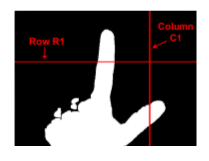
\includegraphics[scale=0.6]{Imgs/BSLCLAS.png}
		\caption{الگوی استخراج ویژگی}
	\end{subfigure}
	\begin{subfigure}{.4\textwidth}
%		\center
		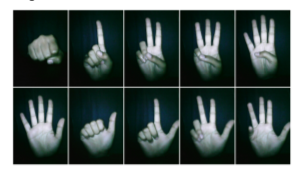
\includegraphics[scale=0.7]{Imgs/BSL.png}
		\caption{ الگوی ارقام زبان ناشنوایان انگلیس}
	\end{subfigure}
	
	\caption{الگوی ارقام در زبان ناشنوایان کشور انگلیس و الگوی استخراج ویژگی در پژوهش \cite{rupanagudi2015high}}

\label{fig:bsl1}
\end{figure}

در پژوهش \cite{panwar2012hand}، با استفاده از قطعه‌بندی تصویر از طریق آستانه‌ای‌سازی، ناحیه‌ای که دست در آن قرار دارد، استخراج می‌شود. سپس با محاسبه طول و عرض این ناحیه و تقسیم آن‌ها بر هم، موقعیت و زاویه دست، محاسبه می‌شود. پس از این مرحله، ویژگی‌هایی از قبیل مرکز ثقل دست و ناحیه انگشتان، از تصویر استخراج شده و در یک بردار ۵ بیتی بازنمایی می‌شود. سپس با استفاده از این بردارهای ویژگی استخراج شده، عمل دسته‌بندی انجام می‌شود. شکل \ref{fig:hsr}، تصاویر مربوط به این مقاله را نمایش می‌دهد.


\begin{figure}[h]
\center
	\begin{subfigure}{.3\textwidth}
%		\center
		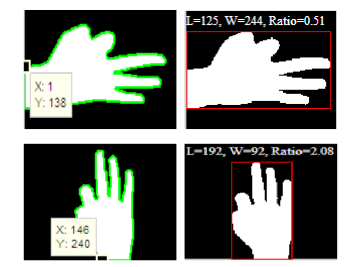
\includegraphics[scale=0.4]{Imgs/hsp1.png}
		\caption{نتیجه قطعه‌بندی و  تشخیص وضعیت}
	\end{subfigure}
	\begin{subfigure}{.4\textwidth}
%		\center
		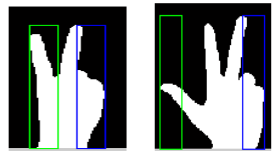
\includegraphics[scale=0.6]{Imgs/hsp2.png}
		\caption{ تشخیص ناحیه انگشتان}
	\end{subfigure}
	\\
	\begin{subfigure}{.5\textwidth}
%		\center
		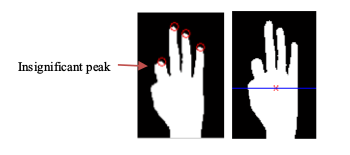
\includegraphics[scale=0.7]{Imgs/hsp3.png}
		\caption{ استخراج ویژگی‌های نوک انگشتان و مرکز ثقل دست}
	\end{subfigure}
	
	\caption{مراحل مختلف پردازش در پژوهش \cite{panwar2012hand}}
	\label{fig:hsr}
\end{figure}

در پژوهش \cite{badi2016recent}، مروری بر فعالیت‌های انجام شده مبتنی بر بینایی رایانه برای تشخیص حالت دست در سال 2016 انجام شده است. هم‌چنین در روش ارائه شده در این پژوهش، پس از قطعه‌بندی تصویر با استفاده از آستانه‌ای‌سازی تصویر و حذف نویز با اعمال پشت سرهم فیلتر میانه\enfootnote{Median Filter}، ناحیه تصویر برای استخراج لبه‌ها به مرحله بعد ارسال می‌شود. استخراج لبه با استفاده از فیلتر سوبل\enfootnote{Sobel Edge Detection Filter}، انجام می‌شود. سپس از یک شبکه عصبی پرسپترونی چندلایه\enfootnote{Multilayer Perceptron Network (MLP)}، برای دسته‌بندی استفاده شده است. شبکه عصبی مورد استفاده در این پژوهش، از 1060 گره در لایه ورودی، 100 گره در لایه مخفی و 6 گره در لایه خروجی با نرخ یادگیری 0.9 تشکیل شده‌است. شکل\ref{fig:hsann} مراحل مختلف اجرای این الگوریتم را نمایش می‌دهد.


\begin{figure}[h]
\center
	\begin{subfigure}{.3\textwidth}
%		\center
		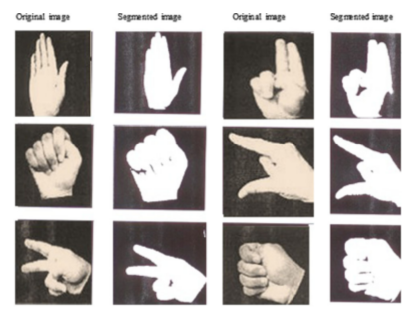
\includegraphics[scale=0.4]{Imgs/hsann1.png}
		\caption{تصاویر ورودی و نتیجه قطعه‌بندی. ستون‌های دوم و چهارم نتایج قطعه‌بندی و ستون‌های اول و سوم تصاویر ورودی هستند.}
	\end{subfigure}
	\begin{subfigure}{.4\textwidth}
%		\center
		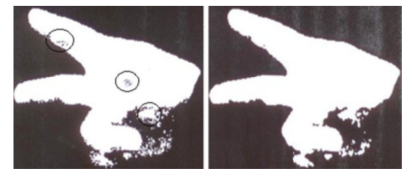
\includegraphics[scale=0.4]{Imgs/hsannn2.png}
		\caption{ حذف نویز}
	\end{subfigure}
	\\
	\begin{subfigure}{.3\textwidth}
%		\center
		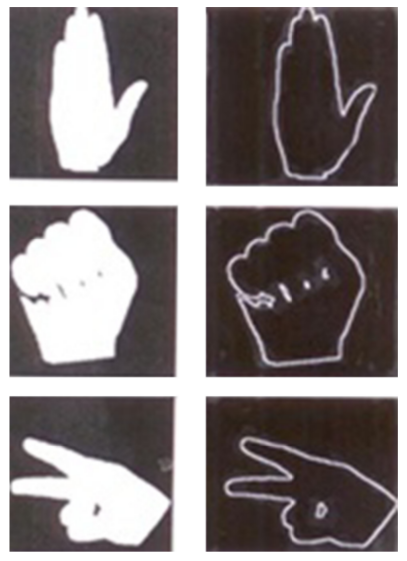
\includegraphics[scale=0.3]{Imgs/hsann3.png}
		\caption{ استخراج لبه‌ها با استفاده از فیلتر سوبل}
	\end{subfigure}
	
	\caption{مراحل مختلف پردازش در پژوهش \cite{badi2016recent}}
	\label{fig:hsr}
\end{figure}

روش‌های مشابه دیگری نیز ارائه شده است که به دلیل پرهیز از بلندگویی، از بیان آن‌ها صرفه‌نظر می‌کنیم. یکی از فعالیت‌های شاخصی که در این زمینه انجام شده است، پژوهش \cite{huang2011gabor} است که با استفاده از اعمال فیلترهای گابور\enfootnote{Gabor Filters}، عمل تشخیص حالت دست را انجام داده است. این پژوهش را به طور مفصل در ادامه بررسی خواهیم نمود.

\subsubsection{استفاده از فیلترهای گابور}	
نتایج پژوهش‌ها نشان می‌دهد، ساختار چشم گربه، سلسله‌مراتبی است و سلول‌های موجود در پایین‌ترین سطح، فقط قادر به استخراج ویژگی‌های بسیار ساده از تصویر هستند. این ویژگی‌های استخراج شده، در سطوح بالاتر، با یک‌دیگر ترکیب می‌شوند و تصویر کلی را می‌سازند. نحوه کار سلول‌های سطح پایین چشم، مشابه اعمال فیلترهای گاوسی در پردازش تصویر است. فیلترهای گابور، فیلترهای گاوسی هستند که در توابع سینوسی کانوالو\enfootnote{Convolve}، شده‌اند. پژوهش‌ها نشان می‌دهند، اعمال این فیلترها در زوایای مختلف، عملکرد بسیار مناسبی در قطعه‌بندی تصاویر دارد.
\\
در پژوهش \cite{huang2011gabor}، از این فیلترها برای تشخیص حالت دست استفاده شده است. در این پژوهش، در مرحله پیش‌پردازش، ابتدا تصویر ورودی، به فضاهای رنگی مختلف نگاشت می‌شود. برای هر فضای رنگی، یک معیار ارزیابی محاسبه می‌شود. در نهایت، تصویر ورودی به فضای رنگی با بیشترین مقدار معیار ارزیابی نگاشت می‌شود و از آن برای مراحل بعدی استفاده می‌شود. این مرحله به دلیل جلوگیری از تاثیر نورهای اضافی موجود در محیط و نویز حاصل از شدت روشنایی انجام می‌شود.
شکل \ref{fig:hpg1} نحوه انجام این محاسبه را نمایش می‌دهد. 

\begin{figure}[h]
\center
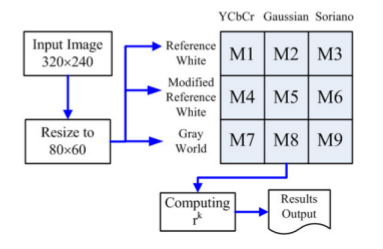
\includegraphics[scale=0.4]{Imgs/hpg1.png}
\caption{انتخاب مناسب‌ترین فضای رنگی برای انجام محاسبات \cite{huang2011gabor}}
\label{fig:hpg1}
\end{figure}

پس از انتخاب بهترین فضای رنگی، فیلترهای گابور را در زوایای مختلف به تصویر اعمال می‌کنیم. شکل\ref{fig:gf}، فیلترهای گابور را در زوایای مختلف نمایش می‌دهد.

\begin{figure}[h]
\center
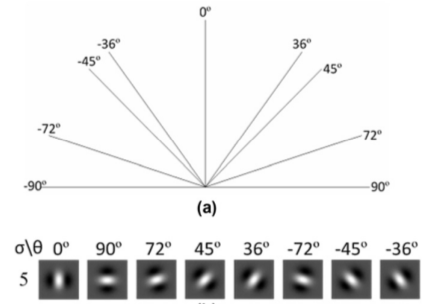
\includegraphics[scale=0.4]{Imgs/gf.png}
\caption{فیلترهای گابور در زوایای مختلف \cite{huang2011gabor}}
\label{fig:gf}
\end{figure}

با اعمال هریک از فیلترها به تصویر در فضای رنگی جدید، برجستگی‌های تصویر در راستای زاویه فیلتر، استخراج می‌شود. شکل \ref{fig:hpg2} نتیجه اعمال این فیلترها را به یکی از تصاویر ورودی نمایش می‌دهد. همان‌طور که مشخص است، در تمام تصاویر بخش‌هایی از دست استخراج شده است و بقیه حواشی تصویر مانند آستین فرد و یا بافت زمینه به طور کامل از تصویر حذف شده‌اند.


\begin{figure}[h]
\center
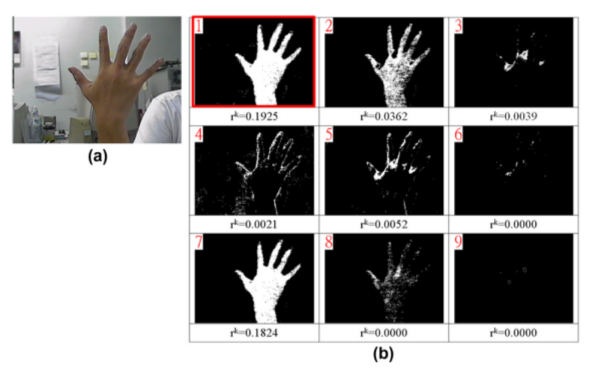
\includegraphics[scale=0.6]{Imgs/gf2.png}
\caption{ نتیجه اعمال فیلترهای گاوسی در زوایای مختلف به تصویر \cite{huang2011gabor}}
\label{fig:gf2}
\end{figure}

پس از استخراج ناحیه دست توسط فیلترهای گابور و قطعه‌بندی تصویر، برای استخراج ویژگی در این پژوهش، با اسکن کردن تصویر از بالا به پایین و در راستای سطرها، هیستوگرام گرادیان\enfootnote{Histogram of Gradient (HoG)} تصویر به عنوان ویژگی‌های کاندید محاسبه می‌شود. شکل\ref{fig:hpgf} هیستوگرام گرادیان یک تصویر را نمایش می‌دهد. سپس با استفاده از الگوریتم  \lr{PCA}، کاهش بعد روی این هیستوگرام انجام شده و ویژگی‌های مفید برای دسته‌بندی استخراج می‌شوند. ویژگی‌های استخراج شده، بعدا با استفاده از دسته‌بندی‌کننده \lr{SVM} دسته‌بندی می‌شوند.


\begin{figure}[h]
\center
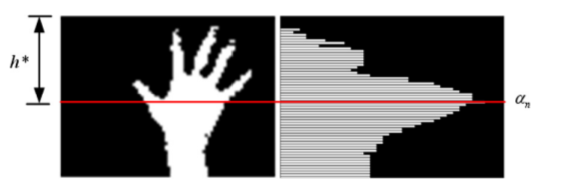
\includegraphics[scale=0.6]{Imgs/hpgf.png}
\caption{محاسبه هیستوگرام تصویر پاسخ فیلترهای گابور به تصویر ورودی \cite{huang2011gabor}}
\label{fig:hpgf}
\end{figure}



%%%%%%%%%%%%%%%%%%%%%%%%%%%%%%%%%%%%%%%%%%%%%%%%%%%%%%%%%%%%%%%%%%%%%%%%%%%%%%%%%%%
\section{ پیاده‌سازی}

در این پروژه، با استفاده از فیلترهای گابور، قطعه‌بندی روی تصویر ورودی انجام می‌شود. سپس با استفاده از ویژگی‌های سیفت\enfootnote{SIFT Features}، تصویر را به بردار ویژگی تبدیل کرده و با استفاده از دسته‌بندی کننده \lr{SVM}، عمل دسته‌بندی را انجام می‌دهیم. در ادامه به بررسی بخش‌های مختلف کد خواهیم پرداخت.
\subsection{پیش‌پردازش داده‌های ورودی}
ابتدا رزولوشن تصویر ورودی را با استفاده از هرم دقت\enfootnote{Resolution Pyramid}، کاهش می‌دهیم. این کار به افزایش سرعت اجرای الگوریتم کمک بسیار زیادی می‌کند. برنامه \ref{prg:pyrd}، بخشی از کد را که این کار را انجام می‌دهد نمایش می‌دهد. این کار را تا زمانی انجام می‌دهیم که ابعاد تصویر ورودی از ابعاد از پیش‌تعیین‌شده‌ای کمتر شود تا مطمئن باشیم الگوریتم، کارایی خود را حفظ خواهد کرد.


 \begin{LTR}
    \begin{lstlisting}[style=C++Style,caption=\rl{کاهش رزولوشن تصویر}]
	Mat input = input_src  ;
	while(input.rows > max_size || input.cols > max_size)
	{
		pyrDown(input_src,input,Size(input_src.cols/2,input_src.rows/2));
		input_src = input ;
	}
    \end{lstlisting}
    \label{prg:gyrd}
  \end{LTR}
  

 در مرحله پیش‌پردازش، ما برخلاف پژوهش \cite{huang2011gabor}، به طور پویا، فضای رنگی مورد استفاده را انتخاب نمی‌کنیم. بلکه در این بخش، ما به طور مشخص، تصاویر ورودی را به فضای رنگی \lr{YCrCb} منتقل می‌کنیم. ویژگی این فضا این است که به طور کامل، روشنایی نقاط را از رنگ آن‌ها جدا می‌کند. با این‌ کار، تصویر ورودی را که در فضای رنگی \lr{RGB} تولید شده است و دارای سه کانال رنگی است به فضای رنگی \lr{YCrCb} که دارای سه کانال رنگی است منتقل می‌کنیم. از این تصویر در مراحل بعد استفاده می‌کنیم. برنامه \ref{prg:cvtcol} بخشی از کد را که انتقال فضای رنگی را انجام می‌دهد، نمایش می‌دهد.
 
 
 \begin{LTR}
    \begin{lstlisting}[style=C++Style,caption=\rl{انتقال فضای رنگی}]
	cout << "converting color space"<<endl;
	cvtColor(input, input, CV_BGR2YCrCb);
	input *= float(1)/255;
    \end{lstlisting}
    \label{prg:cvtcol}
  \end{LTR}

\subsection{اعمال فیلترهای گابور}

در این بخش، فیلترهای گابور را با زوایای مختلف به تصاویر هر یک از کانال‌های تصویر به صورت جداگانه اعمال می‌کنیم. این کار باعث ‌می‌شود متوجه شویم کدام‌یک از کانال‌های موجود، بهترین تفکیک را انجام می‌دهد.
برنامه \ref{prg:gabors}، فیلترهای گابور را در زوایای مختلف به تصویر اعمال می‌کند. این فیلتر ها در زوایای صفر تا $\phi$ با فاصله ۱۵ درجه، اعمال می‌شوند.
  
 \begin{LTR}
    \begin{lstlisting}[style=C++Style,caption=\rl{اعمال فیلترهای گابور در زوایای مختلف به تصویر پیش‌پردازش شده}]
	cout << "filter convolution" <<endl;
	Mat weighted_sum_image (input.rows, input.cols, 21);
	int kernel_size = 3;
	double sig = 1, th = 0, lm = 1.0, gm = 1, ps = 1;
	for (;th <= 180 ; th += 15)
	{
		if(DEBUG)
			cout <<"Theta:" << th << endl;
		Mat kernel = getGaborKernel(Size(kernel_size, kernel_size), sig, th, lm, gm, ps);
		Mat filtered_image ;
		filter2D(input, filtered_image,  CV_32F, kernel);
		addWeighted(weighted_sum_image, 0.5 , filtered_image , 0.5 , 0, weighted_sum_image , weighted_sum_image.type()) ;
	}

	for(int i = 0 ; i < 200 ; i++)
		medianBlur(weighted_sum_image, weighted_sum_image , 3);
	    \end{lstlisting}
    \label{prg:gabors}
  \end{LTR}

همان‌‌طور که مشاهده می‌شود، \textbf{برخلاف تمام پژوهش‌ها}، ما پاسخ فیلترهای مختلف را به صورت جداگانه بررسی نمی‌کنیم. بلکه از آنجایی‌که تمام این فیلترها، نواحی مختلف دست در راستاهای مختلف را برجسته می‌کنند، با تجمیع همه آن‌ها در یک تصویر، تصویر کامل دست را در فضا تشکیل می‌دهیم. شکل \ref{fig:gsfigs} تصاویر حاصل از این مرحله را نمایش می‌دهد.

\begin{figure}[h]
\center
	\begin{subfigure}{.4\textwidth}
%		\center
		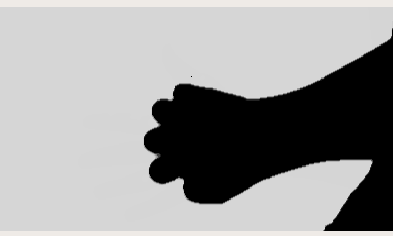
\includegraphics[scale=0.4]{Imgs/gabors1.png}
		\caption{کانال اول از پاسخ گابور}
	\end{subfigure}
	\begin{subfigure}{.4\textwidth}
%		\center
		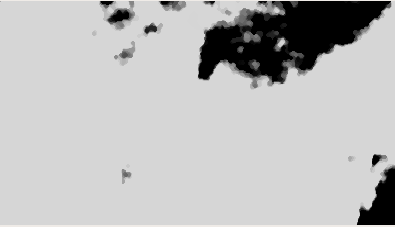
\includegraphics[scale=0.4]{Imgs/gabors2.png}
		\caption{کانال دوم از پاسخ گابور}
	\end{subfigure}
\\
	\begin{subfigure}{.4\textwidth}
%		\center
		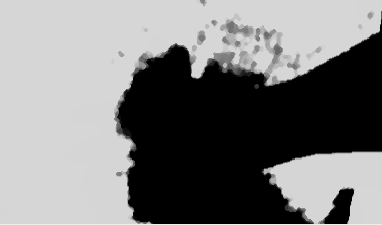
\includegraphics[scale=0.4]{Imgs/gabors3.png}
		\caption{کانال سوم از پاسخ گابور}
	\end{subfigure}
	\begin{subfigure}{.4\textwidth}
%		\center
		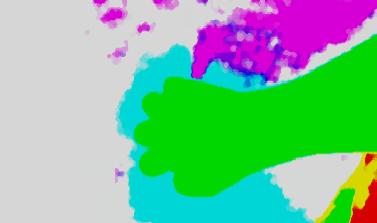
\includegraphics[scale=0.4]{Imgs/gabors4.png}
		\caption{مجموعه سه کانال پاسخ گابور}
	\end{subfigure}
\\
	\begin{subfigure}{.3\textwidth}
%		\center
		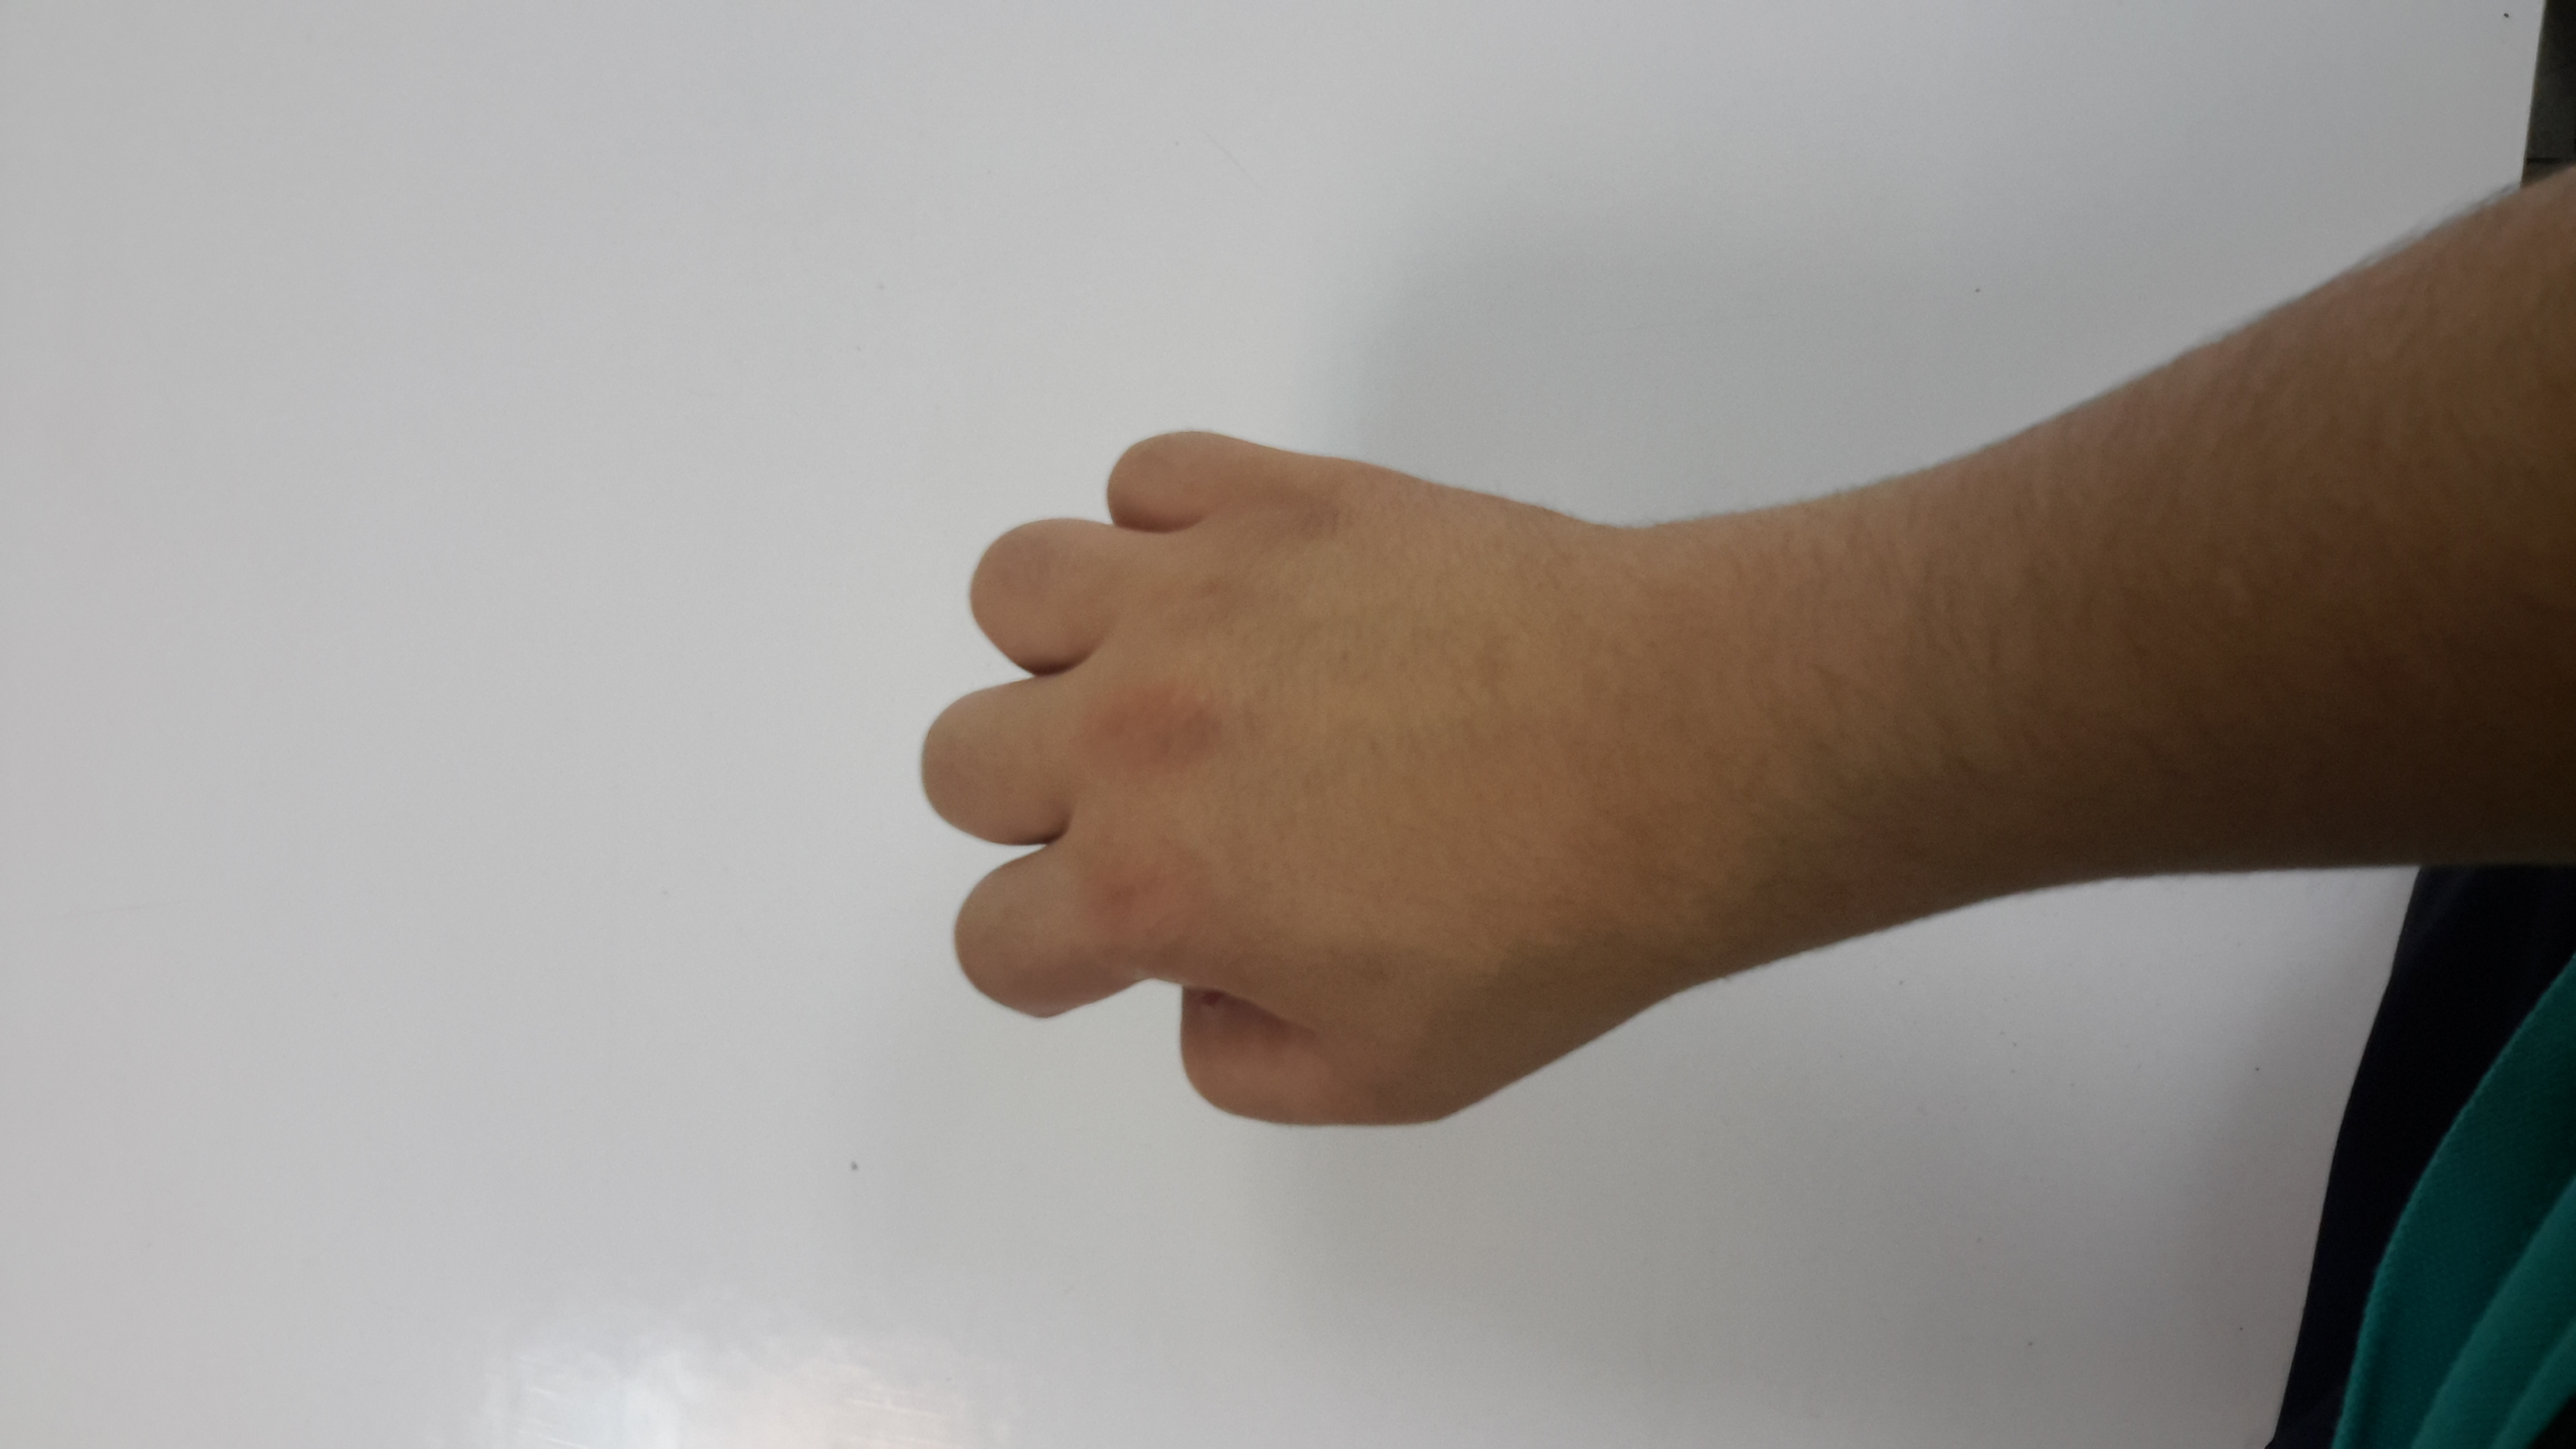
\includegraphics[scale=0.05]{Imgs/origImgGab.jpg}
		\caption{ تصویر ورودی}
	\end{subfigure}
	
	\caption{نتایج اعمال فیلترهای گاوسی در زوایای مختلف و تجمیع پاسخ‌ها}

\label{fig:bsl1}
\end{figure}

همان‌طور که در شکل \ref{fig:gabors} مشخص است، اولین کانال از این پاسخ، بهترین پاسخ ممکن را برای قطعه‌بندی تصویر می‌دهد. در ادامه کار روی خروجی این کانال تمام پردازش‌ها را انجام خواهیم داد.

\subsection{استخراج ویژگی‌های سیفت}
در این مرحله به دنبال یافتن بهترین توصیف‌گرها برای تصاویر هستیم. در ادامه این بخش، مراحل مختلف این کار را مورد بررسی قرار خواهیم داد.

\subsubsection{استخراج نقاط کلیدی}
 برای استخراج نقاط کلیدی از برنامه \ref{prg:sftkpt} استفاده می‌نماییم. در این مرحله ابتدا تصویر ورودی را با یک آستانه‌ای‌سازی ثابت و ساده، آستانه‌ای کرده و سپس به سطح خاکستری تبدیل می‌کنیم. سپس با استفاده از توابع کتابخانه اپن‌سی‌وی\enfootnote{OpenCV}، نقاط کلیدی را استخراج می‌نماییم.

 \begin{LTR}
    \begin{lstlisting}[style=C++Style,caption=\rl{استخراج نقاط کلیدی}]
	image = threshold_and_convert(image);

	SiftFeatureDetector detector;
    vector<KeyPoint> keypoints;
    detector.detect(image, keypoints);
    \end{lstlisting}
    \label{prg:sftkpt}
  \end{LTR}

\subsubsection{محاسبه توصیف‌گر سیفت}
 
 پس از استخراج نقاط کلیدی توسط الگوریتم، می‌توانیم توصیف‌گر تصویر را بسازیم. برنامه \ref{prg:sftdsc}، این توصیف‌گر را برای هر تصویر با استفاده از نقاط کلیدی استخراج شده، محاسبه می‌کند و در قالب یک ماتریس بازنمایی می‌نماید.
 
 
 \begin{LTR}
    \begin{lstlisting}[style=C++Style,caption=\rl{محاسبه توصیف‌گر سیفت}]
 	SiftDescriptorExtractor extractor ;

	Mat descriptor;

	image.convertTo(image, CV_8U);

	extractor.compute(image, keypoints , descriptor);
    \end{lstlisting}
    \label{prg:sftdsc}
  \end{LTR}

 
\subsection{تولید بردار ویژگی با استفاده از ویژگی‌های سیفت استخراج شده}

توصیف‌گر سیفت، یک ماتریس با 128 ستون و به تعداد نقاط کلیدی استخراج شده سطر است. این ماتریس، 128 ویژگی از هر کدام از نقاط کلیدی را مشخص می‌کند. برای تبدیل این توصیف‌گر به یک بردار ویژگی، با توجه به این‌که از هر تصویر تعداد متفاوتی نقطه کلیدی استخراج می‌شود، باید از روش‌های مبتنی بر کیسه کلمات\enfootnote{bag of words} استفاده کنیم. به این منظور، ماتریس توصیف‌گر سیفت را به صورت ستونی جمع می‌کنیم و عملیات نرمال‌سازی را روی هر ستون انجام می‌دهیم. بردار حاصل، بردار ویژگی تولید شده از توصیف‌گر سیفت است. برنامه \ref{prg:ef} کد مربوط به تولید بردار ویژگی را نمایش می‌دهد.


 \begin{LTR}
    \begin{lstlisting}[style=C++Style,caption=\rl{تولید بردار ویژگی}]
		double feature_value[descriptor.cols] ;
		double gamma = 0.05 ;

		for(int j = 0 ; j < descriptor.cols ; j++)
		{
			feature_value[j] = 0 ;
			for(int h = 0 ; h < descriptor.rows ; h++)
			{
				double to_be_added_value = (descriptor.at<double>(h,j)/pow(10,15) ) ;
				feature_value[j] += to_be_added_value;

				if(feature_value[j] > 1)
					feature_value[j] = 1 ;
			}	
		}


		for(int j = 0 ; j < descriptor.cols ; j++)
		{
			if(feature_value[j] < 0 )
				feature_value[j] = 0 ;

			feature_value[j] = 128 * pow(feature_value[j],gamma) ;
			if(DEBUG)
				cout << "feature_value "<< j<<": " << feature_value[j] << endl ; 
		}

		Mat result (1,descriptor.cols, CV_32FC1, feature_value) ;
    \end{lstlisting}
    \label{prg:ef}
  \end{LTR}


\subsection{آموزش دسته‌بندی کننده و استفاده از آن}
آموزش و استفاده از دسته‌بندی کننده برای پیش‌بینی بچسب یک تصویر که به بردار ویژگی نگاشت شده است، با فراخوانی دو تابع، به راحتی انجام می‌شوند.

 \begin{LTR}
    \begin{lstlisting}[style=C++Style,caption=\rl{آموزش دسته‌بندی کننده}]
	training_svm.train(training_data_mat, training_labels_mat, Mat(), Mat(), params);
    \end{lstlisting}
    \label{prg:svmtrn}
  \end{LTR}
  

 \begin{LTR}
    \begin{lstlisting}[style=C++Style,caption=\rl{پیش‌بینی با استفاده از دسته‌بندی‌کننده \lr{SVM}}]
	float predicted_label = svm.predict(feature_vector);
    \end{lstlisting}
    \label{prg:svmtrn}
  \end{LTR}
 
 

%%%%%%%%%%%%%%%%%%%%%%%%%%%%%%%%%%%%%%%%%%%%%%%%%%%%%%%%%%%%%%%%%%%%%%%%%%%%%%%%%%%
\section{ آزمایشات}

مجموعه‌داده مورد آزمایش در این پروژه، مجموعه‌داده مورد استفاده در مقاله \cite{kumar2010hand} است که با استفاده از روش‌های فازی، اقدام به دسته‌بندی تصویر کرده است. در این مجموعه‌داده، 10 کلاس مختلف از حالات دست وجود دارد که در آن از هر دسته حالات، 24 نمونه تصویر وجود دارد. نمونه‌های موجود در هرکدام از کلاس‌های تصویری موجود در این مجموعه‌داده، با تغییر دادن موقعیت و اندازه تصاویر و چرخش‌های جزئی، بوجود آمده‌اند. زمینه تمام تصاویر، ساده و یکنواخت است. شکل\ref{fig:ds}، یک نمونه تصویر از هر کدام از کلاس‌های موجود را نمایش می‌دهد.

\begin{figure}[h]
\center
	\begin{subfigure}{.2\textwidth}
%		\center
		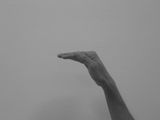
\includegraphics[scale=0.4]{Imgs/ds10.jpg}
		\caption{نمونه تصویر از کلاس اول}
	\end{subfigure}
	\begin{subfigure}{.2\textwidth}
%		\center
		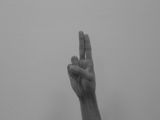
\includegraphics[scale=0.4]{Imgs/ds6.jpg}
		\caption{نمونه تصویر از کلاس دوم}
	\end{subfigure}
	\begin{subfigure}{.2\textwidth}
%		\center
		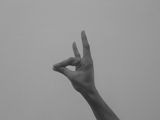
\includegraphics[scale=0.4]{Imgs/ds8.jpg}
		\caption{نمونه تصویر از کلاس سوم}
	\end{subfigure}
	\begin{subfigure}{.2\textwidth}
%		\center
		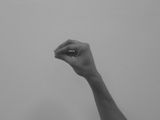
\includegraphics[scale=0.4]{Imgs/ds9.jpg}
		\caption{نمونه تصویر از کلاس چهارم}
	\end{subfigure}
\\
	\begin{subfigure}{.2\textwidth}
%		\center
		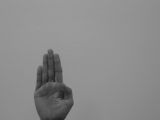
\includegraphics[scale=0.4]{Imgs/ds1.jpg}
		\caption{نمونه تصویر از کلاس پنجم}
	\end{subfigure}
	\begin{subfigure}{.2\textwidth}
%		\center
		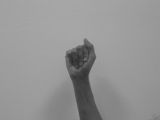
\includegraphics[scale=0.4]{Imgs/ds7.jpg}
		\caption{نمونه تصویر از کلاس ششم}
	\end{subfigure}
	\begin{subfigure}{.2\textwidth}
%		\center
		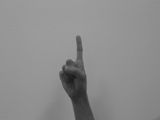
\includegraphics[scale=0.4]{Imgs/ds5.jpg}
		\caption{نمونه تصویر از کلاس هفتم}
	\end{subfigure}
	\begin{subfigure}{.2\textwidth}
%		\center
		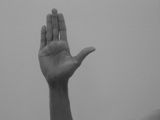
\includegraphics[scale=0.4]{Imgs/ds2.jpg}
		\caption{نمونه تصویر از کلاس هشتم}
	\end{subfigure}
\\
	\begin{subfigure}{.2\textwidth}
%		\center
		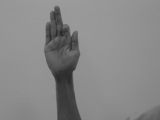
\includegraphics[scale=0.4]{Imgs/ds3.jpg}
		\caption{نمونه تصویر از کلاس نهم}
	\end{subfigure}
	\begin{subfigure}{.2\textwidth}
%		\center
		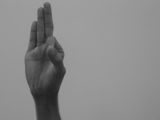
\includegraphics[scale=0.4]{Imgs/ds4.jpg}
		\caption{نمونه تصویر از کلاس دهم}
	\end{subfigure}
\\
	
	\caption{نمونه تصاویر موجود در مجموعه‌داده}

\label{fig:ds}
\end{figure}

جدول \ref{tbl:res}، نتایج اعمال روش پیاده‌سازی‌شده را بر روی مجموعه‌داده مورد استفاده گزارش می‌کند. 

\begin{table}[h]
\center
\caption{نتایج نهایی اعمال روش ارائه شده به مجموعه‌داده}
\label{tbl:res}
\begin{tabular}{c | c | c }
& دقت پیش‌بینی & زمان اجرا برای هر تصویر
\\
\hline
\hline
مجموعه آموزشی& 83.75 & 0.059
\\
مجموعه تست& 33.34& 0.056
\end{tabular}
\end{table}

 همین‌طور جدول \ref{tbl:resdet}، نتیجه پیش‌بینی الگوریتم به ازای هر کدام از کلاس‌ها را به طور جداگانه گزارش 
 می‌دهد. همان‌طور که مشخص است، تصاویر کلاس‌های ۵، 7، ۸، ۹ و ۱۰ بسیار به هم شبیه هستند. این مورد باعث می‌شود،  در زمان آموزش، تعداد ویژگی‌هایی که به کلاس ۱۰ شبیه هستند، زیاد شود. دسته‌بندی‌کننده در مواجهه با چنین مشکلی، بیشتر به سمت کلاس ۱۰ متمایل می‌شود و روی داده‌های این کلاس، به نوعی بیش‌برازش اتفاق می‌افتد. مؤید این نکته این است که در جدول \ref{tbl:resdet}، روی مجموعه‌ تست، دقت این کلاس برابر با ۱۰۰ شده و بقیه کلاس‌ها به شدت پایین هستند. برای حل این مساله باید با اضافه کردن ویژگی یا ویژگی‌هایی که بتواند این کلاس‌ها را از هم متمایز کند، دقت دسته‌بندی را افزایش دهیم. استفاده از الگوریتم‌هایی مانند \lr{PCA} هم که کاهش بعد انجام داده و ویژگی‌های تکراری را از بین می‌برند، می‌تواند بسیار مفید باشد.


\begin{table}[h]
\center
\caption{نتایج نهایی اعمال روش ارائه شده به مجموعه‌داده به تفکیک کلاس‌ها}
\label{tbl:resdet}
\begin{tabular}{c | c | c | c | c | c | c | c | c | c | c}
شماره کلاس & 1 & 2 &3 & 4 & 5 & 6 & 7 & 8 & 9 & 10
\\
\hline
\hline
مجموعه آموزشی& 50 & 75 & 87.5 & 83.34 & 95.84 & 87.5 & 87.5 & 91.67 & 79.16 & 100
\\
مجموعه تست  & 22.23 & 22.23 & 33.34 & 11.12 & 33.34 & 11.12 & 22.23 & 33.34 & 44.45 & 100
\end{tabular}
\end{table}
 
 
%%%%%%%%%%%%%%%%%%%%%%%%%%%%%%%%%%%%%%%%%%%%%%%%%%%%%%%%%%%%%%%%%%%%%%%%%%%%%%%%%%%
\section{ جمع‌بندی}

تشخیص حالت دست، به طور کلی به یکی از دو روش زیر انجام می‌شود:

\begin{enumerate}
\item تشخیص مبتنی بر اسکلت دست
در این دسته از روش‌ها، با استفاده از نظریه تطبیق گراف یا با استفاده از مدل‌های گرافی احتمالی، سعی در بازسازی مدل اسکلت دست در هر تصویر می‌شود. با داشتن مدل اسکلت دست، می‌توان عمل دسته‌بندی را به خوبی انجام داد.
\item تشخیص مبتنی بر مساحت دست
در این دسته از روش‌ها، با استفاده از قطعه‌بندی تصویر و آستانه‌سازی آن و استخراج ویژگی از تصاویر حاصل برای استفاده در دسته‌بندی کننده، می‌تواند منجر به دسته‌بندی تصاویر بر حسب حالات مختلف دست شود.
\end{enumerate}

استفاده از فیلترهای گابور برای برجسته‌کردن نقاط مهم تصویر از جمله روش‌هایی است که در تشخیص مساحت دست بسیار مفید است. روند انجام عملیات در روش ارائه شده در این مقاله به طور خلاصه به شرح زیر است:

\begin{enumerate}
\item انتقال فضای رنگی دست از \lr{RGB} به \lr{YCrCb}
\item کاهش رزولوشن تصویر با استفاده از هرم دقت
\item اعمال فیلترهای گابور به کانال‌های مختلف تصویر و انتخاب بهترین کانال
\item استخراج نقاط کلیدی سیفت
\item استخراج توصیف‌گر سیفت برای تصویر
\item تولید بردار ویژگی بر اساس روش کیسه کلمات از توصیف‌گر سیفت
\item آموزش و استفاده از دسته‌بندی کننده \lr{SVM}
\end{enumerate}

روش ارائه شده در این پروژه، با اضافه کردن ویژگی‌های متمایز کننده کلاس‌های ۷ تا ۱۰ از یک‌دیگر، قابلیت ارتقا عملکرد زیادی دارد.

\newpage
%%%%%%%%%%%%%%%%%%%%%%%%%%%%%%%%%%%%%%%%%%%%%%%%%%%%%%%%%%%%%%%%%%%%%%%%%%%%%%%%%%%
%\vfill
%\section{توضیحات}
%\begin{itemize}
%%\item [*] با توجه به ز مان‌بر بودن اجرای کامل الگوریتم، عموم آزمایشات نتیجه تکرار چهارم و پنجم الگوریتم هستند. بدیهی  است ادامه اجرای الگوریتم بر بهبود پاسخ موثر خواهد بود اما نتایج مقایسات تغییری نخواهند کرد. 
%%\item [*] سورس کد مربوط به پروژه در ضمیمه این گزارش ارسال شده است. همین‌طور این کد از
%%\href{https://github.com/ahmad-asadi/PGM/tree/master/MarkovRandomField}
%%{این لینک}
%%، قابل 
%%دریافت می‌باشد.
%%\item [*] آدرس لینک برای دریافت کد:
%%\LTR{
%%\url{https://github.com/ahmad-asadi/PGM/tree/master/BayesianNetwork}
%%}
%\end{itemize}
%%%%%%%%%%%%%%%%%%%%%%%%%%%%%%%%%%%%%%%%%%%%%%%%%%%%%%%%%%%%%%%%%%%%%%%%%%%%%%%%%%%
\bibliographystyle{acm-fa.bst}
\bibliography{ref}



\end{document} 
